\documentclass{report}
\usepackage[utf8]{inputenc}
\usepackage[T1]{fontenc}
\usepackage{CormorantGaramond}
\usepackage{fontspec}
\usepackage{geometry}
\usepackage[table]{xcolor}
\usepackage{tabularx}
\usepackage{graphicx}
\usepackage{mathtools}
\usepackage[bottom]{footmisc}
\usepackage[italian]{babel}
\usepackage{hyperref}
\usepackage{titlesec}
\usepackage{listings}
\usepackage{color}
\usepackage{graphicx}
\usepackage{fancyhdr}
\usepackage{float}

\graphicspath{{contenuti/images}}

\renewcommand{\headrulewidth}{0.4pt}
\renewcommand{\footrulewidth}{0.4pt}

\lstset{ % General setup for the package
    basicstyle=\small\sffamily,
    numbers=left,
     numberstyle=\tiny,
    frame=tb,
    tabsize=4,
    columns=fixed,
    showstringspaces=false,
    showtabs=false,
    keepspaces,
    commentstyle=\color{red},
    keywordstyle=\color{blue}
}

\geometry{
a4paper,
total = {170mm, 240mm},
left = 20mm,
top = 20mm,
}

\setlength{\headheight}{33.60004pt}

\setlength{\parindent}{0em}
\setlength{\parskip}{0.7em}

\titlespacing*{\section}{0pt}{0.7em}{0.5em}
\titlespacing*{\subsection}{0pt}{0.7em}{0.5em}

\newcommand{\gassets}{../}



\renewcommand{\title}{
    PoC
    
    \tiny Versione documento: \textit{V0.0.1}
}

\newcommand{\people}{
    \normalsize
    \begin{center}
        \begin{tabularx}{7cm}{l | X}            
            \textbf{Uso} & Esterno\\
            \textbf{Destinatario} & Committente\\
            & Cliente \\
        \end{tabularx}
    \end{center}
}

\fancypagestyle{plain}{%
    \fancyhead{} % clear all header fields
    \fancyhead[L]{\leftmark}
    \fancyhead[R]{\textit{SWEasabi} \includegraphics[height=30pt]{\gassets global-assets/img/loghi/SWEasabi_compact_logo.png}}
    \fancyfoot{} % clear all footer fields
    \fancyfoot[L]{\thepage}
    \fancyfoot[R]{Piano di qualifica}
}

\begin{document}

\pagestyle{fancy}

\fancyhead{} % clear all header fields
\fancyhead[L]{\leftmark}
\fancyhead[R]{\textit{SWEasabi} \includegraphics[height=30pt]{\gassets global-assets/img/loghi/SWEasabi_compact_logo.png}}
\fancyfoot{} % clear all footer fields
\fancyfoot[L]{\thepage}
\fancyfoot[R]{Piano di qualifica}


\input{\gassets global-assets/tex/header}
\thispagestyle{empty}
\clearpage
%\pagenumbering{Roman}
%\section{Registro delle modifiche}

%Tabella
\begin{center}
    \begin{tabularx}{\linewidth}{|l|l|X|X|}            
        \hline
        \textbf{Versione} & \textbf{Data} & \textbf{Modifica}& \textbf{Persone}\\
        \vzerozerotre
        \vzerozerodue
        \vzerozerouno
        \hline

    \end{tabularx}
\end{center}

\tableofcontents
\clearpage
\pagenumbering{arabic}
\chapter{Tecnologie}\label{tecnologie}

\begin{itemize}
    \item Angular
    \item Java Spring
    \item Eclipse Mosquitto
    \item Java
\end{itemize}
\chapter{Scopo}\label{scopo}

Lo scopo del POC è quello di dimostrare padronanza di una limitata selezione di tecnologie rilevanti al progetto. In particolare, le principali tecnologie utilizzate sono state Angular per la pagina front-end, Java Spring per l'api REST e Mosquitto come broker mqtt.

\begin{figure}
    
\includegraphics[width=\linewidth]{poc.jpg}
    \caption{Simple visual representation}
\end{figure}
\chapter{API Java Spring}\label{funzionamento}

\section{Introduzione}

Lo scopo dell'API è quello di fornire servizi REST alla pagina angular e comunicare con le applicazioni che vanno a svolgere la logica effettiva del progetto. In particolare, vengono offerte due GET, rispettivamente disponibili su Lamps e Lamps/id, e una PUT, anch'essa su Lamps/id.

Nel progetto sarà presente un'ulteriore separazione tra API e servizi in modo da non esporli all'esterno\footnote{L'API che si occuperà di verificare che la richiesta avvenga da un utente autorizzato e dirigendola verso la corretta applicazione.}. Tuttavia essendo questo PoC puramente a scopo dimostrativo questa caratteristicha non è presente. Come concordato con il proponente, in questo prototipo l'enfasi è stata posta sulla corretta comunicazione tra le diverse parti del progetto, ritenendo il vero e proprio processo di autenticazione superfluo in questo PoC.

\section{Funzionamento}

\subsection{Database}

Per migliorare il funzionamento del PoC, è stato dotato di un piccolo database temporaneo a cui viene fatto un preload di alcune variabili durante l'inizializzazione del programma.

\subsection{Richieste GET}

Il progetto offre due GET, una su lamps e una su lamps/id. Queste GET ritornano rispettivamente i dettagli di tutte le lampade presenti (ad esempio il loro id, dove sono situate, o il loro status, ovvero se si tratta di una lampadina accesa o spenta) o quelli di una singola lampada corrispondente all'id selezionato.

\begin{figure}[H]
    \centering
    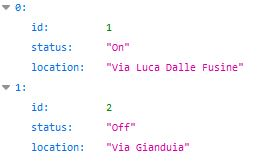
\includegraphics{lamps.jpg}
    \caption{Api risponde a richiesta su /Lamps}
\end{figure}

\begin{figure}[H]
    \centering
    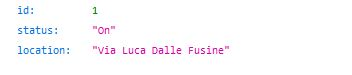
\includegraphics{lampsid.jpg}
    \caption{Api risponde a richiesta su /Lamps/1}
\end{figure}

\subsection{Richiesta PUT}

Come menzionato sopra il progetto offre anche una PUT, anch'essa a Lamps/id. Questo servizio consente di modificare i dettagli della lampadina corrispondente, in particolare di modificare il proprio stato (quindi accenderla o spegnerla).

\begin{figure}[H]
    \centering
    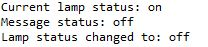
\includegraphics{put1.jpg}
    \caption{Richiesta PUT: La lampadina non è nello stato richiesto}
\end{figure}

\begin{figure}[H]
    \centering
    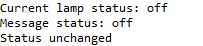
\includegraphics{put2.jpg}
    \caption{Richiesta PUT: La lampadina è già nello stato richiesto}
\end{figure}

\subsection{Comunicazione MQTT}

A ogni richiesta effettuata, l'API posta messaggi sui topic relativi alle lampadine utilizzando mqtt (nel caso del nostro progetto con broker mosquitto), messaggi che vengono successivamente letti dalle nostre applicazioni in back-end. Come spiegato sopra, questo passaggio è essenziale in quanto serve a comunicare con i servizi veri e propri facendogli eseguire le diverse operazioni richieste, tuttavia è più a scopo dimostrativo sul funzionamento della comunicazioni in questo PoC.

\begin{figure}[H]
    \centering
    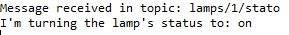
\includegraphics{mqtt.jpg}
    \caption{Richiesta PUT: Client legge il messaggio mqtt in arrivo dall'API}
\end{figure}
\chapter{Angular}\label{angular}

\section{Introduzione}

Lo scopo della pagina web prodotta in Angular, è quello di fornire le operazioni necessarie per attuare la modifica dello stato della lampada, sfruttando le funzionalità dell'API. \\
Nell'ottica del PoC, la modifica è riservata alla lampada con \texttt{id = 1}. \\
L'utente ha la capacità di visualizzare lo stato corrente della lampada, sia in forma visiva che testuale, e di modificarne lo stato. 

\section{Funzionamento}

\subsection{\texttt{lamp-button.component.ts}}
Questo componente consiste di un pulsante che cambia lo stato di una lampada. Visualizza inoltre un'immagine della lampada (Figura \ref{fig:getlamps}), variabile in base allo stato, e il suo stato corrente in forma testuale.

\subsection{All'avvio della pagina - \texttt{ngOnInit()}}
All'avvio della pagina web, viene invocato il metodo \texttt{getStatus()}.\\
Il metodo \texttt{getStatus()} è responsabile di ottenere lo stato corrente della lampada tramite una chiamata GET, ed aggiornare il valore locale nel BehaviorSubject \texttt{lampStatus\$} con il nuovo stato.

\subsection{\texttt{getStatus()}}
Questo metodo recupera lo stato corrente della lampada attraverso una chiamata GET all'endpoint \footnote[1]{Definizione di endpoint : 
Gli endpoint sono dispositivi fisici che si connettono e scambiano informazioni con una rete di computer. Alcuni esempi di endpoint sono dispositivi mobili, computer desktop, macchine virtuali, dispositivi incorporati e server.} (/lamps/1). \\

\subsection{Al tocco della lampada - \texttt{toggleLamp()}}

Si offre il metodo \texttt{toggleLamp()}, tale metodo cambia lo stato della lampada tramite una chiamata PUT, da un valore locale "On", ad "Off", e viceversa.

\section{Template HTML}
Il template HTML mostra un'immagine della lampada ed il suo stato corrente. \\
Tale immagine è anche un pulsante che chiama il metodo \texttt{toggleLamp()}, quando viene cliccata o premuta (Figura \ref{fig:modifylamps}).

\section{Metodi di supporto}

\subsection{\texttt{getData\$()}}
Si offre il metodo \texttt{getData\$()}, il quale effettua una richiesta HTTP GET all'endpoint API (/lamps/1), per recuperare lo stato corrente della lampada.

\subsection{\texttt{toggleLamp\$()}}
Questo metodo effettua una richiesta HTTP PUT all'endpoint API (/lamps/1), per cambiare lo stato della lampada. \\
Prende un parametro "status" che rappresenta lo stato corrente della lampada. \\
Se lo stato è "On", invia una modifica del parametro in "Off" per spegnere la lampada, e viceversa.

\section{Immagini}

\begin{figure}[H]
    \centering
    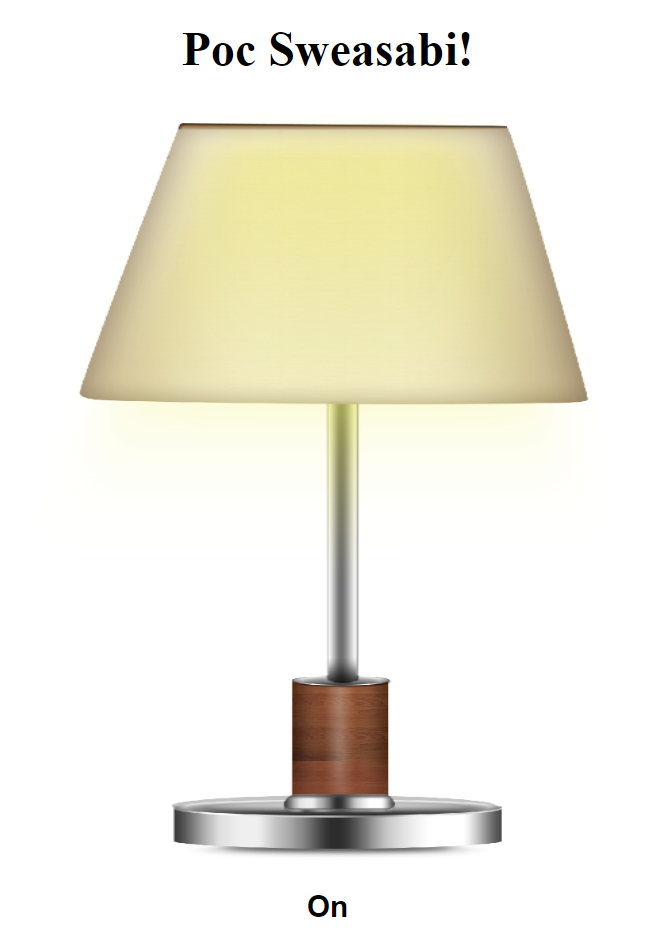
\includegraphics[width=0.5\linewidth]{getlamps.png}
    \caption{Button fa richiesta di stato iniziale su /Lamps/1}
    \label{fig:getlamps}
\end{figure}


\begin{figure}[H]
    \centering
    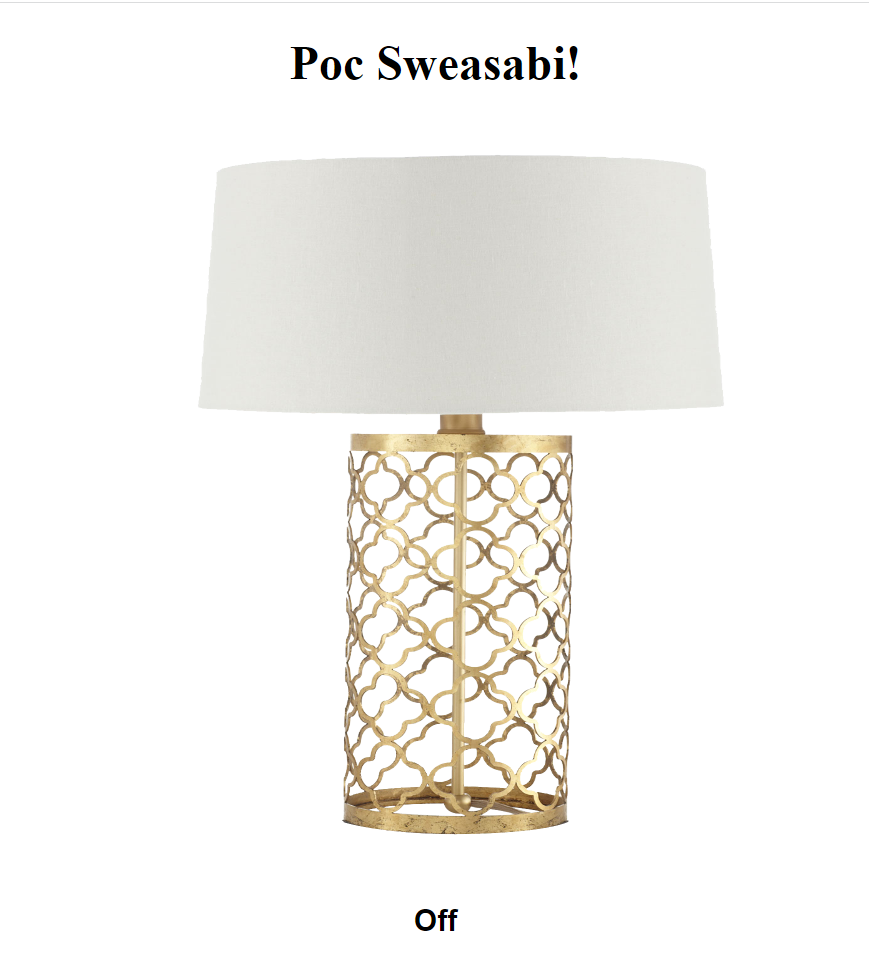
\includegraphics[width=0.6\linewidth]{modifylamps.png}
    \caption{Button fa cambio di stato su /Lamps/1}
    \label{fig:modifylamps}
\end{figure}

\end{document}
